
%% bare_jrnl.tex
%% V1.4a
%% 2014/09/17
%% by Michael Shell
%% see http://www.michaelshell.org/
%% for current contact information.
%%
%% This is a skeleton file demonstrating the use of IEEEtran.cls
%% (requires IEEEtran.cls version 1.8a or later) with an IEEE
%% journal paper.
%%
%% Support sites:
%% http://www.michaelshell.org/tex/ieeetran/
%% http://www.ctan.org/tex-archive/macros/latex/contrib/IEEEtran/
%% and
%% http://www.ieee.org/

%%*************************************************************************
%% Legal Notice:
%% This code is offered as-is without any warranty either expressed or
%% implied; without even the implied warranty of MERCHANTABILITY or
%% FITNESS FOR A PARTICULAR PURPOSE! 
%% User assumes all risk.
%% In no event shall IEEE or any contributor to this code be liable for
%% any damages or losses, including, but not limited to, incidental,
%% consequential, or any other damages, resulting from the use or misuse
%% of any information contained here.
%%
%% All comments are the opinions of their respective authors and are not
%% necessarily endorsed by the IEEE.
%%
%% This work is distributed under the LaTeX Project Public License (LPPL)
%% ( http://www.latex-project.org/ ) version 1.3, and may be freely used,
%% distributed and modified. A copy of the LPPL, version 1.3, is included
%% in the base LaTeX documentation of all distributions of LaTeX released
%% 2003/12/01 or later.
%% Retain all contribution notices and credits.
%% ** Modified files should be clearly indicated as such, including  **
%% ** renaming them and changing author support contact information. **
%%
%% File list of work: IEEEtran.cls, IEEEtran_HOWTO.pdf, bare_adv.tex,
%%                    bare_conf.tex, bare_jrnl.tex, bare_conf_compsoc.tex,
%%                    bare_jrnl_compsoc.tex, bare_jrnl_transmag.tex
%%*************************************************************************


% *** Authors should verify (and, if needed, correct) their LaTeX system  ***
% *** with the testflow diagnostic prior to trusting their LaTeX platform ***
% *** with production work. IEEE's font choices and paper sizes can       ***
% *** trigger bugs that do not appear when using other class files.       ***                          ***
% The testflow support page is at:
% http://www.michaelshell.org/tex/testflow/



%\documentclass[journal]{IEEEtran}
\documentclass[12pt, draftclsnofoot, onecolumn]{IEEEtran}
%
% If IEEEtran.cls has not been installed into the LaTeX system files,
% manually specify the path to it like:
% \documentclass[journal]{../sty/IEEEtran}
\usepackage[latin1]{inputenc}
\usepackage{amsfonts}
\usepackage{amssymb}
\usepackage{amsthm}
\usepackage{fullpage}
\usepackage{setspace}
\usepackage{graphicx}
%\usepackage[pdftex]{graphicx}
\usepackage{psfrag}
\usepackage{color}
\usepackage{epsfig}
%\usepackage{appendix}
%\usepackage{caption}
%\usepackage{cite}
%\usepackage{ifpdf}
%\usepackage[cmex10]{amsmath}
\usepackage{algorithm}
%\usepackage{array}
%\usepackage{stfloats}
\usepackage{url}
%\usepackage{fixltx2e}
\usepackage{setspace} 
\usepackage{diagbox}
\usepackage{subfigure}
\usepackage{algpseudocode}
\usepackage{multirow}
\usepackage{calc}




% Some very useful LaTeX packages include:
% (uncomment the ones you want to load)


% *** MISC UTILITY PACKAGES ***
%
\usepackage{ifpdf}
% Heiko Oberdiek's ifpdf.sty is very useful if you need conditional
% compilation based on whether the output is pdf or dvi.
% usage:
% \ifpdf
%   % pdf code
% \else
%   % dvi code
% \fi
% The latest version of ifpdf.sty can be obtained from:
% http://www.ctan.org/tex-archive/macros/latex/contrib/oberdiek/
% Also, note that IEEEtran.cls V1.7 and later provides a builtin
% \ifCLASSINFOpdf conditional that works the same way.
% When switching from latex to pdflatex and vice-versa, the compiler may
% have to be run twice to clear warning/error messages.






% *** CITATION PACKAGES ***
%
\usepackage{cite}
% cite.sty was written by Donald Arseneau
% V1.6 and later of IEEEtran pre-defines the format of the cite.sty package
% \cite{} output to follow that of IEEE. Loading the cite package will
% result in citation numbers being automatically sorted and properly
% "compressed/ranged". e.g., [1], [9], [2], [7], [5], [6] without using
% cite.sty will become [1], [2], [5]--[7], [9] using cite.sty. cite.sty's
% \cite will automatically add leading space, if needed. Use cite.sty's
% noadjust option (cite.sty V3.8 and later) if you want to turn this off
% such as if a citation ever needs to be enclosed in parenthesis.
% cite.sty is already installed on most LaTeX systems. Be sure and use
% version 5.0 (2009-03-20) and later if using hyperref.sty.
% The latest version can be obtained at:
% http://www.ctan.org/tex-archive/macros/latex/contrib/cite/
% The documentation is contained in the cite.sty file itself.






% *** GRAPHICS RELATED PACKAGES ***
%
\ifCLASSINFOpdf
  % \usepackage[pdftex]{graphicx}
  % declare the path(s) where your graphic files are
  % \graphicspath{{../pdf/}{../jpeg/}}
  % and their extensions so you won't have to specify these with
  % every instance of \includegraphics
  % \DeclareGraphicsExtensions{.pdf,.jpeg,.png}
\else
  % or other class option (dvipsone, dvipdf, if not using dvips). graphicx
  % will default to the driver specified in the system graphics.cfg if no
  % driver is specified.
  % \usepackage[dvips]{graphicx}
  % declare the path(s) where your graphic files are
  % \graphicspath{{../eps/}}
  % and their extensions so you won't have to specify these with
  % every instance of \includegraphics
  % \DeclareGraphicsExtensions{.eps}
\fi
% graphicx was written by David Carlisle and Sebastian Rahtz. It is
% required if you want graphics, photos, etc. graphicx.sty is already
% installed on most LaTeX systems. The latest version and documentation
% can be obtained at: 
% http://www.ctan.org/tex-archive/macros/latex/required/graphics/
% Another good source of documentation is "Using Imported Graphics in
% LaTeX2e" by Keith Reckdahl which can be found at:
% http://www.ctan.org/tex-archive/info/epslatex/
%
% latex, and pdflatex in dvi mode, support graphics in encapsulated
% postscript (.eps) format. pdflatex in pdf mode supports graphics
% in .pdf, .jpeg, .png and .mps (metapost) formats. Users should ensure
% that all non-photo figures use a vector format (.eps, .pdf, .mps) and
% not a bitmapped formats (.jpeg, .png). IEEE frowns on bitmapped formats
% which can result in "jaggedy"/blurry rendering of lines and letters as
% well as large increases in file sizes.
%
% You can find documentation about the pdfTeX application at:
% http://www.tug.org/applications/pdftex





% *** MATH PACKAGES ***
%
\usepackage[cmex10]{amsmath}
% A popular package from the American Mathematical Society that provides
% many useful and powerful commands for dealing with mathematics. If using
% it, be sure to load this package with the cmex10 option to ensure that
% only type 1 fonts will utilized at all point sizes. Without this option,
% it is possible that some math symbols, particularly those within
% footnotes, will be rendered in bitmap form which will result in a
% document that can not be IEEE Xplore compliant!
%
% Also, note that the amsmath package sets \interdisplaylinepenalty to 10000
% thus preventing page breaks from occurring within multiline equations. Use:
%\interdisplaylinepenalty=2500
% after loading amsmath to restore such page breaks as IEEEtran.cls normally
% does. amsmath.sty is already installed on most LaTeX systems. The latest
% version and documentation can be obtained at:
% http://www.ctan.org/tex-archive/macros/latex/required/amslatex/math/





% *** SPECIALIZED LIST PACKAGES ***
%
%\usepackage{algorithmic}
% algorithmic.sty was written by Peter Williams and Rogerio Brito.
% This package provides an algorithmic environment fo describing algorithms.
% You can use the algorithmic environment in-text or within a figure
% environment to provide for a floating algorithm. Do NOT use the algorithm
% floating environment provided by algorithm.sty (by the same authors) or
% algorithm2e.sty (by Christophe Fiorio) as IEEE does not use dedicated
% algorithm float types and packages that provide these will not provide
% correct IEEE style captions. The latest version and documentation of
% algorithmic.sty can be obtained at:
% http://www.ctan.org/tex-archive/macros/latex/contrib/algorithms/
% There is also a support site at:
% http://algorithms.berlios.de/index.html
% Also of interest may be the (relatively newer and more customizable)
% algorithmicx.sty package by Szasz Janos:
% http://www.ctan.org/tex-archive/macros/latex/contrib/algorithmicx/




% *** ALIGNMENT PACKAGES ***
%
\usepackage{array}
% Frank Mittelbach's and David Carlisle's array.sty patches and improves
% the standard LaTeX2e array and tabular environments to provide better
% appearance and additional user controls. As the default LaTeX2e table
% generation code is lacking to the point of almost being broken with
% respect to the quality of the end results, all users are strongly
% advised to use an enhanced (at the very least that provided by array.sty)
% set of table tools. array.sty is already installed on most systems. The
% latest version and documentation can be obtained at:
% http://www.ctan.org/tex-archive/macros/latex/required/tools/


% IEEEtran contains the IEEEeqnarray family of commands that can be used to
% generate multiline equations as well as matrices, tables, etc., of high
% quality.




% *** SUBFIGURE PACKAGES ***
%\ifCLASSOPTIONcompsoc
%  \usepackage[caption=false,font=normalsize,labelfont=sf,textfont=sf]{subfig}
%\else
%  \usepackage[caption=false,font=footnotesize]{subfig}
%\fi
% subfig.sty, written by Steven Douglas Cochran, is the modern replacement
% for subfigure.sty, the latter of which is no longer maintained and is
% incompatible with some LaTeX packages including fixltx2e. However,
% subfig.sty requires and automatically loads Axel Sommerfeldt's caption.sty
% which will override IEEEtran.cls' handling of captions and this will result
% in non-IEEE style figure/table captions. To prevent this problem, be sure
% and invoke subfig.sty's "caption=false" package option (available since
% subfig.sty version 1.3, 2005/06/28) as this is will preserve IEEEtran.cls
% handling of captions.
% Note that the Computer Society format requires a larger sans serif font
% than the serif footnote size font used in traditional IEEE formatting
% and thus the need to invoke different subfig.sty package options depending
% on whether compsoc mode has been enabled.
%
% The latest version and documentation of subfig.sty can be obtained at:
% http://www.ctan.org/tex-archive/macros/latex/contrib/subfig/




% *** FLOAT PACKAGES ***
%
%\usepackage{fixltx2e}
% fixltx2e, the successor to the earlier fix2col.sty, was written by
% Frank Mittelbach and David Carlisle. This package corrects a few problems
% in the LaTeX2e kernel, the most notable of which is that in current
% LaTeX2e releases, the ordering of single and double column floats is not
% guaranteed to be preserved. Thus, an unpatched LaTeX2e can allow a
% single column figure to be placed prior to an earlier double column
% figure. The latest version and documentation can be found at:
% http://www.ctan.org/tex-archive/macros/latex/base/


%\usepackage{stfloats}
% stfloats.sty was written by Sigitas Tolusis. This package gives LaTeX2e
% the ability to do double column floats at the bottom of the page as well
% as the top. (e.g., "\begin{figure*}[!b]" is not normally possible in
% LaTeX2e). It also provides a command:
%\fnbelowfloat
% to enable the placement of footnotes below bottom floats (the standard
% LaTeX2e kernel puts them above bottom floats). This is an invasive package
% which rewrites many portions of the LaTeX2e float routines. It may not work
% with other packages that modify the LaTeX2e float routines. The latest
% version and documentation can be obtained at:
% http://www.ctan.org/tex-archive/macros/latex/contrib/sttools/
% Do not use the stfloats baselinefloat ability as IEEE does not allow
% \baselineskip to stretch. Authors submitting work to the IEEE should note
% that IEEE rarely uses double column equations and that authors should try
% to avoid such use. Do not be tempted to use the cuted.sty or midfloat.sty
% packages (also by Sigitas Tolusis) as IEEE does not format its papers in
% such ways.
% Do not attempt to use stfloats with fixltx2e as they are incompatible.
% Instead, use Morten Hogholm'a dblfloatfix which combines the features
% of both fixltx2e and stfloats:
%
 \usepackage{dblfloatfix}
% The latest version can be found at:
% http://www.ctan.org/tex-archive/macros/latex/contrib/dblfloatfix/




%\ifCLASSOPTIONcaptionsoff
%  \usepackage[nomarkers]{endfloat}
% \let\MYoriglatexcaption\caption
% \renewcommand{\caption}[2][\relax]{\MYoriglatexcaption[#2]{#2}}
%\fi
% endfloat.sty was written by James Darrell McCauley, Jeff Goldberg and 
% Axel Sommerfeldt. This package may be useful when used in conjunction with 
% IEEEtran.cls'  captionsoff option. Some IEEE journals/societies require that
% submissions have lists of figures/tables at the end of the paper and that
% figures/tables without any captions are placed on a page by themselves at
% the end of the document. If needed, the draftcls IEEEtran class option or
% \CLASSINPUTbaselinestretch interface can be used to increase the line
% spacing as well. Be sure and use the nomarkers option of endfloat to
% prevent endfloat from "marking" where the figures would have been placed
% in the text. The two hack lines of code above are a slight modification of
% that suggested by in the endfloat docs (section 8.4.1) to ensure that
% the full captions always appear in the list of figures/tables - even if
% the user used the short optional argument of \caption[]{}.
% IEEE papers do not typically make use of \caption[]'s optional argument,
% so this should not be an issue. A similar trick can be used to disable
% captions of packages such as subfig.sty that lack options to turn off
% the subcaptions:
% For subfig.sty:
% \let\MYorigsubfloat\subfloat
% \renewcommand{\subfloat}[2][\relax]{\MYorigsubfloat[]{#2}}
% However, the above trick will not work if both optional arguments of
% the \subfloat command are used. Furthermore, there needs to be a
% description of each subfigure *somewhere* and endfloat does not add
% subfigure captions to its list of figures. Thus, the best approach is to
% avoid the use of subfigure captions (many IEEE journals avoid them anyway)
% and instead reference/explain all the subfigures within the main caption.
% The latest version of endfloat.sty and its documentation can obtained at:
% http://www.ctan.org/tex-archive/macros/latex/contrib/endfloat/
%
% The IEEEtran \ifCLASSOPTIONcaptionsoff conditional can also be used
% later in the document, say, to conditionally put the References on a 
% page by themselves.




% *** PDF, URL AND HYPERLINK PACKAGES ***
%
\usepackage{url}
% url.sty was written by Donald Arseneau. It provides better support for
% handling and breaking URLs. url.sty is already installed on most LaTeX
% systems. The latest version and documentation can be obtained at:
% http://www.ctan.org/tex-archive/macros/latex/contrib/url/
% Basically, \url{my_url_here}.




% *** Do not adjust lengths that control margins, column widths, etc. ***
% *** Do not use packages that alter fonts (such as pslatex).         ***
% There should be no need to do such things with IEEEtran.cls V1.6 and later.
% (Unless specifically asked to do so by the journal or conference you plan
% to submit to, of course. )


% correct bad hyphenation here
%\hyphenation{op-tical net-works semi-conduc-tor}


\begin{document}
%
% paper title
% Titles are generally capitalized except for words such as a, an, and, as,
% at, but, by, for, in, nor, of, on, or, the, to and up, which are usually
% not capitalized unless they are the first or last word of the title.
% Linebreaks \\ can be used within to get better formatting as desired.
% Do not put math or special symbols in the title.
\title{Progress Report}
%
%
% author names and IEEE memberships
% note positions of commas and nonbreaking spaces ( ~ ) LaTeX will not break
% a structure at a ~ so this keeps an author's name from being broken across
% two lines.
% use \thanks{} to gain access to the first footnote area
% a separate \thanks must be used for each paragraph as LaTeX2e's \thanks
% was not built to handle multiple paragraphs
%

%\author{Michael~Shell,~\IEEEmembership{Member,~IEEE,}
  %      John~Doe,~\IEEEmembership{Fellow,~OSA,}
 %       and~Jane~Doe,~\IEEEmembership{Life~Fellow,~IEEE}% <-this % stops a space
%\thanks{M. Shell is with the Department
%of Electrical and Computer Engineering, Georgia Institute of Technology, Atlanta,
%GA, 30332 USA e-mail: (see http://www.michaelshell.org/contact.html).}% <-this % stops a space
%\thanks{J. Doe and J. Doe are with Anonymous University.}% <-this % stops a space
%\thanks{Manuscript received April 19, 2005; revised September 17, 2014.}}

\author{Tianpei Chen\\
Department of Electrical and Computer Engineering\\
McGill University\\
Montreal, Quebec, Canada}

% note the % following the last \IEEEmembership and also \thanks - 
% these prevent an unwanted space from occurring between the last author name
% and the end of the author line. i.e., if you had this:
% 
% \author{....lastname \thanks{...} \thanks{...} }
%                     ^------------^------------^----Do not want these spaces!
%
% a space would be appended to the last name and could cause every name on that
% line to be shifted left slightly. This is one of those "LaTeX things". For
% instance, "\textbf{A} \textbf{B}" will typeset as "A B" not "AB". To get
% "AB" then you have to do: "\textbf{A}\textbf{B}"
% \thanks is no different in this regard, so shield the last } of each \thanks
% that ends a line with a % and do not let a space in before the next \thanks.
% Spaces after \IEEEmembership other than the last one are OK (and needed) as
% you are supposed to have spaces between the names. For what it is worth,
% this is a minor point as most people would not even notice if the said evil
% space somehow managed to creep in.



% The paper headers
%\markboth{Journal of \LaTeX\ Class Files,~Vol.~13, No.~9, September~2014}%
%{Shell \MakeLowercase{\textit{et al.}}: Bare Demo of IEEEtran.cls for Journals}
% The only time the second header will appear is for the odd numbered pages
% after the title page when using the twoside option.
% 
% *** Note that you probably will NOT want to include the author's ***
% *** name in the headers of peer review papers.                   ***
% You can use \ifCLASSOPTIONpeerreview for conditional compilation here if
% you desire.




% If you want to put a publisher's ID mark on the page you can do it like
% this:
%\IEEEpubid{0000--0000/00\$00.00~\copyright~2014 IEEE}
% Remember, if you use this you must call \IEEEpubidadjcol in the second
% column for its text to clear the IEEEpubid mark.



% use for special paper notices
%\IEEEspecialpapernotice{(Invited Paper)}




% make the title area
\maketitle

% As a general rule, do not put math, special symbols or citations
% in the abstract or keywords.
\begin{abstract}
The abstract goes here.
\end{abstract}

% Note that keywords are not normally used for peerreview papers.
\begin{IEEEkeywords}
IEEEtran, journal, \LaTeX, paper, template.
\end{IEEEkeywords}






% For peer review papers, you can put extra information on the cover
% page as needed:
% \ifCLASSOPTIONpeerreview
% \begin{center} \bfseries EDICS Category: 3-BBND \end{center}
% \fi
%
% For peerreview papers, this IEEEtran command inserts a page break and
% creates the second title. It will be ignored for other modes.
\IEEEpeerreviewmaketitle



\section{System Model}
% The very first letter is a 2 line initial drop letter followed
% by the rest of the first word in caps.
% 
% form to use if the first word consists of a single letter:
% \IEEEPARstart{A}{demo} file is ....
% 
% form to use if you need the single drop letter followed by
% normal text (unknown if ever used by IEEE):
% \IEEEPARstart{A}{}demo file is ....
% 
% Some journals put the first two words in caps:
% \IEEEPARstart{T}{his demo} file is ....
% 
% Here we have the typical use of a "T" for an initial drop letter
% and "HIS" in caps to complete the first word.
%\IEEEPARstart{T}{his} demo file is intended to serve as a ``starter file''
%for IEEE journal papers produced under \LaTeX\ using
%IEEEtran.cls version 1.8a and later.
% You must have at least 2 lines in the paragraph with the drop letter
% (should never be an issue)
%I wish you the best of success.

%\hfill mds
 
%\hfill September 17, 2014
Consider an uncoded complex Large-Scale MIMO (LS-MIMO) uplink spatial multiplexing (SM) system with $N_{t}$ users, each is equipped with one transmit antenna. The number of receive antennas at the Base Station (BS) is $N_{r}$. Typically LS-MIMO systems have hundreds of antennas at the BS, 
%as shown in Fig {\ref{large MIMO uplink model}}.
 % \begin{figure}[htb]
  %\centering
  %\def\svgwidth{\columnwidth}
  %\includegraphics[scale=•]{•}
 % \input{largeMIMOuplink.pdf_tex}
  %\caption{Large MIMO uplink system }
  %\label{large MIMO uplink model}
  %\end{figure}
    
Bit sequences, which are modulated to complex symbols, are transmitted by the users over a flat fading channel. The discrete time model of the system is given by:
\begin{equation}
\mathbf{y}=\mathbf{H}\mathbf{s}+\mathbf{n},   \label{discrete time MIMO system}
\end{equation}
where $\mathbf{y}\in\mathbb{C}^{N_{r}\times 1}$ is the received symbol vector, $\mathbf{s}\in \mathbb{C}^{N_{t}\times 1}$ is the transmitted symbol vector, with components that are mutually independent and taken from a finite signal constellation alphabet $\mathbb{O}$ (e.g., BPSK, 4-QAM, 16-QAM, 64-QAM), $|\mathbb{O}|=M$. The transmitted symbol vectors $\mathbf{s}\in \mathbb{O}^{N_{t}}$, satisfy $\mathbb{E}[\mathbf{s}\mathbf{s}^{H}]=\mathbf{I}_{N_t}E_{s}$, where $E_{s}$ denotes the symbol average energy, $\mathbb{E}[\cdot]$ denotes the expectation operation, $\mathbf{I}_{N_{t}}$ denotes identity matrix of size $N_{t}\times N_{t}$. Furthermore $\mathbf{H}\in \mathbb{C}^{N_{r}\times N_{t}}$ denotes the Rayleigh fading channel propagation matrix. $\mathbf{H}_{ij}$ denotes the component of $\mathbf{H}$ at $i$th row and $j$th column, representing the channel response from $i$th receive antenna to the $j$th transmit antenna. Each component is independent identically distributed (i.i.d) circularly symmetric complex Gaussian (CSCG) random variable with unit variance, denoted by $\mathbf{H}_{ij}\sim \mathbb{C}N(0,1)$. Finally, $\mathbf{n}\in \mathbb{C}^{N_{r}}$ is the additive white Gaussian noise (AWGN) vector with zero mean components and $\mathbb{E}[\mathbf{n}\mathbf{n}^{H}]=\mathbf{I}_{N_{r}}N_{0}$, where $N_{0}$ denotes the noise power spectrum density, and hence $\frac{E_{s}}{N_{0}}$ is the symbol signal to noise ratio (SNR). 

The task of a MIMO detector is to estimate the transmit symbol vector $\mathbf{s}$, based on the knowledge of receive symbol vector $\mathbf{y}$ and channel state information (CSI) $\mathbf{H}$. Then a constellation demapper maps each component of $\hat{\mathbf{s}}$ to the corresponding bit sequences. The resulting $N_{t}$ substreams are finally multiplexed to obtain the reconstructed information sequence.

The optimal (in a sense of lowest average frame error probability) Maximum Likelihood Detector (MLD) for MIMO system is given by
\begin{equation}
\hat{\mathbf{s}}^{ML}=\arg\min_{\hat{\mathbf{s}}\in \mathbb{O}^{N_{t}}}||\mathbf{y}-\mathbf{H}\hat{\mathbf{s}}||^{2},
\label{MLD}
\end{equation}
where $||\cdot||$ denotes the 2-norm operation. From (\ref{MLD}), the solution of MLD is the $\hat{\mathbf{s}}$ that can generate the minimum Euclidean distance between vector $\mathbf{y}$ and $\mathbf{H}\hat{\mathbf{s}}$.

Consider an alternative representation of MLD principle, let $\mathbf{H}_{1}\in \mathbb{C}^{N_{r}\times N}$ denotes a sub matrix composed of $N$ columns from $\mathbf{H}$, where $1\leq N\leq N_{t}$, let $\mathbf{s}_{1}\in \mathbb{C}^{N}$ denote the sub symbol vector whose components are transmitted from the users corresponding to $\mathbf{H}_{1}$. Similarly, let $\mathbf{H}_{2}\in \mathbb{C}^{N_{r}\times (N_{t}-N)}$ denotes the sub matrix composed of the remaining columns from $\mathbf{H}$ and $\mathbf{s}_{2}\in \mathbb{C}^{(N_{t}-N)}$ is the sub symbol vector whose components are transmitted by the users corresponding to $\mathbf{H}_{2}$. Thus (\ref{discrete time MIMO system}) can be rewritten as 
\begin{equation}
\mathbf{y}=\mathbf{H}_{1}\mathbf{s}_{1}+\mathbf{H}_{2}\mathbf{s}_{2}+\mathbf{n}.
\label{alternative MIMO system}
\end{equation}  
Let $\hat{\mathbf{s}}_{1}, \hat{\mathbf{s}}_{2}$ denote the estimations of $\mathbf{s}_{1}, \mathbf{s}_{2}$, we have $\hat{\mathbf{s}}_{1}\in [\hat{\mathbf{s}}^{1}_{1}, \hat{\mathbf{s}}^{2}_{1}, \cdots \hat{\mathbf{s}}^{K}_{1}],, K=M^{N}$ and $\hat{\mathbf{s}}_{2}\in [\hat{\mathbf{s}}^{1}_{2}, \hat{\mathbf{s}}^{2}_{2}, \cdots \hat{\mathbf{s}}^{Q}_{2}], Q=M^{N_{t}-N}$, MLD in (\ref{MLD}) can be rewritten as 
\begin{equation}
[\tilde{k}, \tilde{q}]=\arg\min_{k\in [1,2\ldots K]}\min_{q\in [1,2,\ldots, Q]}||\mathbf{y}-\mathbf{H}_{1}\hat{\mathbf{s}}^{k}_{1}-\mathbf{H}_{2}\hat{\mathbf{s}}^{q}_{2}||^{2},\\
\mathbf{s}^{ML}_{1}=\hat{\mathbf{s}}^{\tilde{k}}_{1}, \mathbf{s}^{ML}_{2}=\hat{\mathbf{s}}^{\tilde{q}}_{2},
\label{alternative MLD}
\end{equation}
(\ref{alternative MLD}) can be divided into three steps, first define 
\begin{equation}
\mathbf{y}^{k}=\mathbf{y}-\mathbf{H}_{1}\hat{\mathbf{s}}^{k}_{1}\quad k\in [1,2,\ldots, K],
\label{first step alternative MLD}
\end{equation}
Then solve 
\begin{equation}
\hat{\mathbf{x}}_{2}^{k}=\arg\min_{\hat{\mathbf{s}}_{2}^{q}\in [\hat{\mathbf{s}}_{2}^{1},\hat{\mathbf{s}}_{2}^{3}\ldots, \hat{\mathbf{s}}_{2}^{Q}]}||\mathbf{y}^{k}-\mathbf{H}_{2}\hat{\mathbf{s}}_{2}^{q}||^{2}, 
\label{second step alternative MLD}
\end{equation}
\begin{equation}
\tilde{k}=\arg\min_{k\in [1,2,\ldots, K]}||\mathbf{y}^{k}-\mathbf{H}_{2}\hat{\mathbf{x}}_{2}^{k}||^{2},
\label{third step alternative MLD}
\end{equation}
Finally we have $\mathbf{s}_{1}^{ML}=\hat{\mathbf{s}}_{1}^{\tilde{k}}, \mathbf{s}_{2}^{ML}=\hat{\mathbf{x}}_{2}^{\tilde{k}}=\hat{\mathbf{s}}_{2}^{\tilde{q}}$.
% needed in second column of first page if using \IEEEpubid
%\IEEEpubidadjcol




% An example of a floating figure using the graphicx package.
% Note that \label must occur AFTER (or within) \caption.
% For figures, \caption should occur after the \includegraphics.
% Note that IEEEtran v1.7 and later has special internal code that
% is designed to preserve the operation of \label within \caption
% even when the captionsoff option is in effect. However, because
% of issues like this, it may be the safest practice to put all your
% \label just after \caption rather than within \caption{}.
%
% Reminder: the "draftcls" or "draftclsnofoot", not "draft", class
% option should be used if it is desired that the figures are to be
% displayed while in draft mode.
%
%\begin{figure}[!t]
%\centering
%\includegraphics[width=2.5in]{myfigure}
% where an .eps filename suffix will be assumed under latex, 
% and a .pdf suffix will be assumed for pdflatex; or what has been declared
% via \DeclareGraphicsExtensions.
%\caption{Simulation results for the network.}
%\label{fig_sim}
%\end{figure}

% Note that IEEE typically puts floats only at the top, even when this
% results in a large percentage of a column being occupied by floats.


% An example of a double column floating figure using two subfigures.
% (The subfig.sty package must be loaded for this to work.)
% The subfigure \label commands are set within each subfloat command,
% and the \label for the overall figure must come after \caption.
% \hfil is used as a separator to get equal spacing.
% Watch out that the combined width of all the subfigures on a 
% line do not exceed the text width or a line break will occur.
%
%\begin{figure*}[!t]
%\centering
%\subfloat[Case I]{\includegraphics[width=2.5in]{box}%
%\label{fig_first_case}}
%\hfil
%\subfloat[Case II]{\includegraphics[width=2.5in]{box}%
%\label{fig_second_case}}
%\caption{Simulation results for the network.}
%\label{fig_sim}
%\end{figure*}
%
% Note that often IEEE papers with subfigures do not employ subfigure
% captions (using the optional argument to \subfloat[]), but instead will
% reference/describe all of them (a), (b), etc., within the main caption.
% Be aware that for subfig.sty to generate the (a), (b), etc., subfigure
% labels, the optional argument to \subfloat must be present. If a
% subcaption is not desired, just leave its contents blank,
% e.g., \subfloat[].


% An example of a floating table. Note that, for IEEE style tables, the
% \caption command should come BEFORE the table and, given that table
% captions serve much like titles, are usually capitalized except for words
% such as a, an, and, as, at, but, by, for, in, nor, of, on, or, the, to
% and up, which are usually not capitalized unless they are the first or
% last word of the caption. Table text will default to \footnotesize as
% IEEE normally uses this smaller font for tables.
% The \label must come after \caption as always.
%
%\begin{table}[!t]
%% increase table row spacing, adjust to taste
%\renewcommand{\arraystretch}{1.3}
% if using array.sty, it might be a good idea to tweak the value of
% \extrarowheight as needed to properly center the text within the cells
%\caption{An Example of a Table}
%\label{table_example}
%\centering
%% Some packages, such as MDW tools, offer better commands for making tables
%% than the plain LaTeX2e tabular which is used here.
%\begin{tabular}{|c||c|}
%\hline
%One & Two\\
%\hline
%Three & Four\\
%\hline
%\end{tabular}
%\end{table}


% Note that the IEEE does not put floats in the very first column
% - or typically anywhere on the first page for that matter. Also,
% in-text middle ("here") positioning is typically not used, but it
% is allowed and encouraged for Computer Society conferences (but
% not Computer Society journals). Most IEEE journals/conferences use
% top floats exclusively. 
% Note that, LaTeX2e, unlike IEEE journals/conferences, places
% footnotes above bottom floats. This can be corrected via the
% \fnbelowfloat command of the stfloats package.

\section{Minimum Achievable Diversity based Channel Partition}
\subsection{Diversity Maximization Selection}\label{DMS analysis}
Based on the alternative form of MLD in (\ref{alternative MLD})-(\ref{third step alternative MLD}), General Parallel Interference Cancellation (GPIC) algorithm first generate a list of symbol vector candidates and then choose the candidate with the minimum Euclidean distance as the solution. To elaborate further, GPIC detectors first generate a list of symbol vector candidate by exhaustive search for all the possible $\hat{\mathbf{s}}_{1}$ as shown in (\ref{first step alternative MLD}), then rather than performing exhaustive search in (\ref{second step alternative MLD}), GPIC detectors exploit the low complexity sub optimal linear detectors (i.e., zeros forcing (ZF) and minimum mean square error (MMSE)) and their successive interference cancellation (SIC) counterparts to get the estimation of $\mathbf{s}^{k}_{2}$, $k=[1,2,\ldots, K]$. For sake of simplicity, hereinafter we use LD/SIC. Then the best candidate in the list with the minimum Euclidean distance is chosen as the solution. 

Performance analysis of GPIC algorithm is provided in \cite{radji2009interference}, here we briefly conclude the main results in \cite{radji2009interference}. At the receiving side, the frame error (detection error) is defined as there is at least one erroneous symbol in the estimation of transmitted symbol vector. Let $P_{e}$ denotes the average frame error probability. The diversity order, denoted by $d$ is defined as the slope of the $P_{e}$ in log-scale in high SNR region, which is given by\cite{zheng2003diversity}
\begin{equation}
d=-\lim_{SNR\to\infty}\frac{\log{P_{e}}}{\log(SNR)},
\label{diversity}
\end{equation}
Let $P_{e}^{ML}$ denotes the average frame error probability of MLD, The average frame error probability of GPIC algorithm $P_{et}=\mathbb{E}_{\mathbf{H}, \mathbf{s}}[Pr(\hat{\mathbf{s}}\neq \mathbf{s}|\mathbf{H}, \mathbf{s})]$ and $P_{e2}=\mathbb{E}_{\mathbf{H}_{2}, \mathbf{s}_{2}}(Pr(\hat{\mathbf{s}}^{k_{1}}_{2}\neq \mathbf{s}_{2}|\mathbf{H}_{2}, \mathbf{s}_{2}))$, where $P_{r}(A)$ denotes the probability that a event A occurs, $\hat{\mathbf{s}}_{1}^{k_{1}}=\mathbf{s}_{1}$, therefore $P_{e2}$ is the average frame error probability of the LD/SICs for the sub system in which the interference from the users that transmitted $\mathbf{s}_{1}$ are perfectly cancelled from the observation $\mathbf{y}$. given by
\begin{equation}
\mathbf{y}^{k_{1}}=\mathbf{y}-\mathbf{H}_{1}\hat{\mathbf{s}}_{1}^{k_{1}},
\label{perfect IC}
\end{equation} 
because $\hat{\mathbf{s}}^{k1}_{1}=\mathbf{s}_{1}$, we have
\begin{equation}
\mathbf{y}^{k1}=\mathbf{H}_{2}\mathbf{s}_{2}+\mathbf{H}_{1}(\mathbf{s}_{1}-\hat{\mathbf{s}}_{1}^{k1})+\mathbf{n}=\mathbf{H}_{2}\mathbf{s}_{2}+\mathbf{n},
\label{sub MIMO system}
\end{equation} 
Based on \cite{radji2009interference}, $P_{et}$ is bounded by 
\begin{equation}
\max(P^{ML}_{e}, P_{e2})\leq P_{et}\leq P^{ML}_{e}+P_{e2}, 
\label{average frame error probability of GPIC}
\end{equation}
in (\ref{average frame error probability of GPIC}), the diversity order of MLD is $N_{r}$. Let $d_{t}$ denote the overall diversity order of GPIC detectors and $d_{2}$ denote the diversity order of LD/SICs with the interferences from $\mathbf{s}_{1}$ perfectly cancelled, based on (\ref{diversity}), we have 
\begin{equation}
\lim_{SNR\to\infty}P^{ML}_{e}\propto SNR^{-N_{r}},
\label{MLD diversity}
\end{equation}
\begin{equation}
\lim_{SNR\to\infty}P_{et}\propto SNR^{-d_{t}},
\label{GPIC diversity}
\end{equation}
\begin{equation}
\lim_{SNR\to\infty}P_{e2}\propto SNR^{-d_{2}},
\label{LD diversity}
\end{equation}
 now consider the following conditions
\begin{itemize}
\item $d_{2}>N_{r}$,
\begin{equation}
\lim_{SNR\to\infty}\frac{P_{e2}}{P^{ML}_{e}}=SNR^{N_{r}-d_{2}}=0,
\label{condition1sub1}
\end{equation}
based on (\ref{average frame error probability of GPIC}), we have
\begin{equation}
\lim_{SNR\to\infty}\frac{P_{et}}{P^{ML}_{e}}=1,
\label{condition1sub2}
\end{equation}
thus $d_{t}=N_{r}$.
\item $d_2=N_{r}$,
we have 
\begin{equation}
\lim_{SNR\to\infty}P_{et}\propto SNR^{-N_{r}},
\label{condition2sub1}
\end{equation}
thus $d_{t}=N_{r}$.
\item $d_{2}<N_{r}$,
\begin{equation}
\lim_{SNR\to\infty}\frac{P^{ML}_{e}}{P_{e2}}=SNR^{d_{2}-N_{r}}=0,
\label{condition3sub1}
\end{equation}
based on (\ref{average frame error probability of GPIC}), we have  
\begin{equation}
\lim_{SNR\to\infty}P_{et}=P_{e2}\propto SNR^{-d_{2}},
\label{condition3sub2}
\end{equation}
thus 
$d_{t}=d_{2}$.
\end{itemize} 
Therefore when $d_{2}\geq N_{r}$, GPIC algorithm can achieve ML performance asymptotically, when $d_{2}<N_{r}$, the diversity order that GPIC can achieve at high SNR region is equal to that of LD/SICs. In \cite{radji2009interference}, the authors employ diversity maximization selection (DMS) scheme for channel partition, which is originally proposed in \cite{zhang2006diversity}. The optimal diversity order can be guaranteed with low complexity for conventional small MIMO systems.

To elaborate further, for a given number of antennas chosen at the channel partition stage $N$, there are $N_{u}={N_{t}\choose N}$ possible combinations of $[\mathbf{H}_{1}, \mathbf{H}_{2}]$. According to DMS principle, the maximum diversity order of LD/SIC is achieved by choosing the subset $\mathbf{H}_{2}$ that has the strongest weakest substream, in a sense of post processing SNR. Therefore, when using LD/SIC detectors as the sub optimal detector, the subset $\mathbf{H}^{opt}_{2}$ selected based on DMS principle should be\cite{zhang2006diversity} 
\begin{IEEEeqnarray}[\relax]{l}
\mathbf{H}^{opt}_{2}=\mathbf{H}^{p}_{2},\\
p=\arg\min_{j=1,2,\ldots, N_{u}}\theta_{j},\\
\theta_{j}=\max_{k=1,2,\ldots, N_{t}-N}((\mathbf{H}_{2}^{j})^{H}\mathbf{H}_{2}^{j}+SNR^{-1}\mathbf{I})_{kk}^{-1},\quad \mathbf{H}_{2}^{j}\in[\mathbf{H}_{2}^{1}, \mathbf{H}_{2}^{2}, \ldots, \mathbf{H}_{2}^{N_{u}}];
\label{DMS principle}
\end{IEEEeqnarray}   
Where $\mathbf{A}_{kk}$ denotes the $k$th diagonal component of matrix $\mathbf{A}$. The diversity order of LD/SIC detector after DMS channel partition process is given by 
$d_{2DMS}=(N+1)(N_{r}-N_{t}+N+1)$. In \cite{radji2009interference}, the authors derive the minimum number of antennas $N_{min}$ at channel partition stage that can guarantee $d_{2DMS}\geq N_{r}$, which is given by 
\begin{equation}
N_{min}=\lceil \sqrt{\frac{(N_{r}-N_{t})^{2}}{4}+N_{r}}-\frac{N_{r}-N_{t}}{2}-1\rceil,
\label{Nmin DMS}
\end{equation}
where $\lceil\alpha\rceil$ denotes the minimum integer no less than $\alpha$.
\subsection{Minimum Achievable Diversity: How many transmit antennas do we need to chose in LS-MIMO?}
In LS-MIMO V-BLAS systems, where the substreams are transmitted independently, the maximum diversity order is $N_{r}$, which is extremely large under the condition that there are tens to hundreds of receive antennas. On the one hand, diversity order is achieved at high SNR region, however, in practical, such a high diversity order is not necessary, because the SNR region of interest is the range in which the bit error rate (BER) or symbol error rate (SER) can be $10^{-5}$ to $10^{-7}$. On the other hand, the computational complexity to guarantee ML performance by DMS channel partition is excessive in LS-MIMO, for example, when $N_{r}=N_{t}$, based on (\ref{Nmin DMS}), the $N_{min}=\lceil\sqrt{N_{r}}-1\rceil$, the number of the symbol vector candidates in the list is $M^{N_{min}}$.

Therefore, here we consider minimum achievable diversity (MAD) principle, which can reduce the detection complexity by sacrificing redundant asymptotic diversity gain in LS-MIMO. Let $d_{2MAD}$ denote the diversity order achieved by the suboptimal detectors after the MAD principle based channel partition, $\tilde{N}_{min}$ denote the minimum number of antennas chosen by MAD principle. Our goal is to guarantee the overall diversity is no less than a given minimum diversity while keep $\tilde{N}_{min}$ small. Let $1\leq g<N_{r}$ denote the given minimum achievable diversity order, based on (\ref{condition3sub2}) and the corresponding analysis in section \ref{DMS analysis}, we have
\begin{IEEEeqnarray}[\relax]{l}
\nonumber
 if \quad d_{2MAD}<N_{r}\quad and\quad d_{2MAD}\geq g\\
  d_{t}=d_{2MAD}\geq g.
\end{IEEEeqnarray}
Therefore we can guarantee that the overall diversity order of GPIC algorithm is no less than $g$, in order to derive the minimum number of antennas required based on MAD principle, we define function
\begin{IEEEeqnarray}[\relax]{l}
f(N)=d_{2MAD}-g=(N+1)(N_{r}-N_{t}+N+1)-g,\label{diversity function}
\end{IEEEeqnarray}    
where $N\in [1,2,\ldots, N_{t}]$, our goal is to find minimum $N$, that satisfy $f(N)\geq 0$. The two zero points of quadratic function $f(N)$ are 
\begin{IEEEeqnarray}[\relax]{l}
N_{1}=-\sqrt{\frac{(N_{r}-N_{t})^{2}}{4}+g}-\frac{N_{r}-N_{t}}{2}-1,\\
N_{2}=\sqrt{\frac{(N_{r}-N_{t})^{2}}{4}+g}-\frac{N_{r}-N_{t}}{2}-1
\label{zeros points}
\end{IEEEeqnarray}
when $N\leq N_{1}$ or $N\geq N_{2}$, $f(N)\geq 0$, obviously $N_{1}<0$, there is no feasible $N$ exits that can make the former condition satisfied. Thus, we have 
\begin{equation}
\tilde{N}_{min}=\lceil \sqrt{\frac{(N_{r}-N_{t})^{2}}{4}+g}-\frac{N_{r}-N_{t}}{2}-1\rceil
\label{Nmin MAD}
\end{equation}
\subsection{Computer Simulations}
In this section, computer simulation results for the bit error rate (BER) performances of MAD principle based GPIC algorithm are presented. As a comparison, Sel-MMSE-OSIC algorithm in \cite{radji2009interference} is also considered, denoted by maximum diversity selection (MDS) scheme. The software testbed is built by C, compiled by GCC compiler version 4.9.2 on 64 bit Debian (release 8.2) Linux systems, the experiments are performed on two desktops, one with Intel I5-4th generation CPU, quad cores, 3.2GHz clock rate and the other one with Intel I7-5th generation CPU, six cores, 3.5GHz clock rate.

We consider uncoded complex spatial multiplexing LS-MIMO systems, For each receive SNR point, the BER are calculated with minimum $10^{5}$ independent channel realizations achieved and minimum 300 symbol errors accumulated. The modulation schemes considered are rectangular M-QAM(4-QAM and 16-QAM) with Gray code labeling. In each channel realization, $N_{t}$ mutually independent randomly generated bit sequences are modulated to complex symbols. $N_{t}$ complex symbols are transmitted over randomly generated Rayleigh flat fading channel, each channel matrix component is CSCG random variable with unit variance. The receive symbol vector is corrupted by AWGN.

For sake of simplicity, we use MAD-n to present the results for minimum achievable diversity selection, where $n$ denotes the minimum achievable diversity. The minimum number of antennas selected by channel partition for a given minimum achievable diversity $g$ is given by (\ref{Nmin MAD}). Maximum diversity selection (MDS) is used to present the Sel-MMSE-OSIC that can achieve ML diversity asymptotically. The minimum number of antennas selected in MDS is given by (\ref{Nmin DMS}).

First, we consider $16\times 16$ system with $4$-QAM modulation, Table.\ref{t16MIMO4QAM} shows the information of the schemes considered, the corresponding results are presented in Fig.\ref{f16MIMO4QAM}, 
\begin{table}[htb]
\renewcommand{\arraystretch}{1.3}
\caption{$16\times 16$ system}
\label{t16MIMO4QAM}
\centering
\begin{tabular}{|c|c|c|}
\hline
Scheme&number of antennas selected ($N$)&Asymptotic diversity\\
\hline 
MDS&3&16\\
\hline
MAD-9&2&9\\
\hline
MAD-4&1&4\\
\hline
\end{tabular}
\end{table}

As shown in Fig.\ref{f16MIMO4QAM}, compared with MDS which can achieve ML performance asymptotically, MAD-9 has a small performance loss. While MAD-4's performance is inferior compared to MDS. At BER $10^{-5}$, the MAD-9 is about $0.8$dB worse than MDS, MAD-4 is about $1.8$dB worse than MDS, let $\kappa(\cdot)$ denote the number of symbol vector candidates in the list generated by GPIC algorithm\cite{radji2009interference}, from Table.\ref{t16MIMO4QAM}, 
we have $\frac{\kappa(MAD-9)}{\kappa(DMS)}=1/4$ and $\frac{\kappa(MAD-4)}{\kappa(DMS)}=1/16$.

\begin{figure}[htb]
\centering
%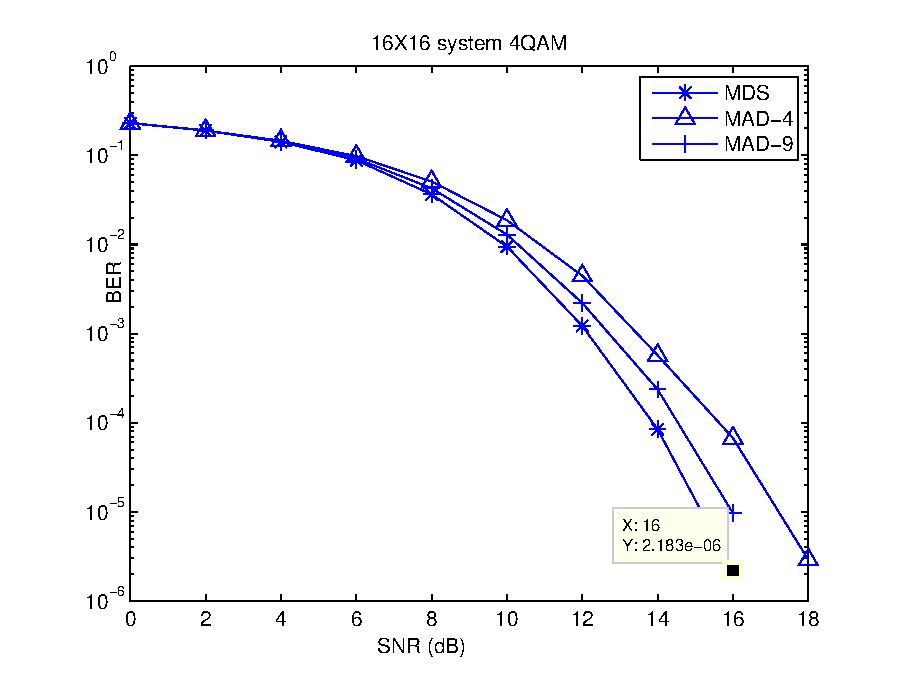
\includegraphics[width=\textwidth]{16MIMO4QAM.eps}
\def\svgwidth{\columnwidth}
\input{16MIMO4QAM.pdf_tex}
\caption{$16\times 16$ system $4$-QAM}
\label{f16MIMO4QAM}
\end{figure}

The results for $16\times 16$ system with $16$-QAM modulation are shown in Fig.\ref{f16MIMO16QAM}, the information of the schemes considered is as the same as that in Talbe.\ref{t16MIMO4QAM}. From Fig.\ref{f16MIMO16QAM}, we can see that similar to the case of $4$-QAM system, MAD-9 has a very small performance loss comparing to DMS, at BER $2\times 10^{-5}$, MAD-9 is about $1.1$dB worse than MDS, while MAD-4 has about $3$dB  performance loss comparing to DMS.

Furthermore, compared with $4$-QAM systems, the reduction of the number of list candidates provided by MAD scheme is more significant in $16$-QAM systems, $\frac{\kappa(MAD-9)}{\kappa(DMS)}=1/16$ and $\frac{\kappa(MAD-4)}{\kappa(DMS)}=1/256$.
\begin{figure}[htb]
\centering
\def\svgwidth{\columnwidth}
\input{16MIMO16QAM.pdf_tex}
\caption{$16\times 16$ system $16$-QAM}
\label{f16MIMO16QAM}
\end{figure}


\begin{table}[htb]
\renewcommand{\arraystretch}{1.3}
\caption{$32\times 32$ system $4$-QAM}
\label{t32MIMO4QAM}
\centering
\begin{tabular}{|c|c|c|}
\hline
Scheme&number of antennas selected ($N$)&Asymptotic diversity\\
\hline 
MAD-4&1&4\\
\hline
MAD-9&2&9\\
\hline
MAD-16&3&16\\
\hline
\end{tabular}
\end{table}

\begin{figure}[htb]
\centering
\def\svgwidth{\columnwidth}
\input{32MIMO4QAM.pdf_tex}
\caption{$32\times 32$ system $4$-QAM}
\label{f32MIMO4QAM}
\end{figure}
Now we consider the performance of MAD in large systems, Fig.\ref{f32MIMO4QAM} shows the results for $32\times 32$ system with $4$-QAM, Table.\ref{t32MIMO4QAM} shows the information of the schemes. Due to the time limitation, we just provide the results for MAD. As we can see in Fig.\ref{f32MIMO4QAM}, although the asymptotic diversity of MAD-16 is much higher than that of MAD-9, at the BER region of interest, their performance difference is negligible. At BER=$3\times 10^{-4}$, the performance of MAD-9 is about $0.3$dB worse comparing to MAD-16, at BER=$3\times 10^{-5}$, the performance loss of MAD-9 is about $0.5$dB comparing to MAD-16.


 
\section{Theoretical Analysis of Channel Hardening Phenomenon}
\subsection{Preliminary}
Orthogonality deficiency $\phi_{od}$ measures the orthogonality of a matrix\cite{ma2008performance}, which is defined by
\begin{equation}
\phi_{od}=1-\frac{det(\mathbf{W})}{\prod_{i=1}^{N_{t}}||\mathbf{h}_{i}||^{2}},
\label{OD}
\end{equation}
where $\mathbf{W}=\mathbf{H}^{H}\mathbf{H}$ denotes Wishart matrix, $\mathbf{h}_{i}$ denotes the $i$ th column of $\mathbf{H}$, $det(\cdot)$ denotes determinant operation, $||\cdot||$ denotes 2-norm operation. Based on Hadamard's inequality $\prod_{i=1}^{N_{t}}||\mathbf{h}_{i}||\geq det(\mathbf{H})$, we have $0\leq\phi_{od}\leq 1$, if $\mathbf{H}$ is singular, $\phi_{od}=1$, if $\mathbf{H}$ is orthogonal, then $\phi_{od}=0$.

$||\mathbf{h}_{i}||^{2}=\sum_{j=1}^{N_{r}}|\mathbf{H}_{ji}|^{2}$, where $|\cdot|$ denotes magnitude operation. $\mathbf{H}_{ij}\sim \mathbb{C}N(0,1)$, where $\mathbb{C}N(0, \sigma^{2})$ denotes CSCG distribution with variance $\sigma^{2}$, thus $|\mathbf{H}_{ji}|\sim Rayleigh(1/\sqrt{2})$, where $Rayleigh(\sigma)$ denotes the Rayleigh distribution with shape parameter $\sigma$, therefore $||\mathbf{h}_{i}||^{2}\sim Gamma(N_{r},1)$\cite{papoulis2002probability}. $Gamma(k,\theta)$ denotes Gamma distribution, with $k$ degrees of freedom and scale parameter $\theta$.

For sake of simplicity, we define orthogonality measure $\phi_{om}$, which is given by 
\begin{equation}
\phi_{om}=\frac{det(\mathbf{W})}{\prod_{i=1}^{N_{t}}||\mathbf{h}_{i}||^{2}},
\label{OM}
\end{equation}
$0\leq \phi_{om}\leq 1$, $\forall \mathbf{H}$, if $\phi_{om}$ is closer to 1, $\mathbf{H}$ is more closer to an orthogonal matrix. 
%\subsection{Introduction to Channel Hardening Phenomenon}
\subsection{Logarithmic Expectation of Orthogonality Measure}
Based on (\ref{OM}), The logarithm of $\phi_{om}$ can be written as 
\begin{equation}
\ln(\phi_{om})=\ln(det(\mathbf{W}))-\sum_{i=1}^{N_{t}}\ln(||\mathbf{h}_{i}||^{2}),
\label{log OM}
\end{equation}
Taking expectation of (\ref{log OM}), we have 
\begin{equation}
\mathbb{E}[\ln(\phi_{om})]=\mathbb{E}[\ln(det(\mathbf{W}))]-\sum_{i=1}^{N_{t}}\mathbb{E}[\ln(||\mathbf{h}_{i}||^{2})].
\label{log expectation OM}
\end{equation}
First we consider the first summand on the right hand of (\ref{log expectation OM}), $\mathbb{E}[\ln(det(\mathbf{W}))]$. Let $\mathbb{C}W_{m}(n, \Sigma)$ denote complex Wishart distribution, which is the joint distribution of sample covariance matrix from multivariate complex Gaussian random variable\cite{goodman1963statistical}. $n$ is the degree of freedom and $\Sigma\in \mathbb{C}^{m\times m}$ is the covariance matrix. Let $\Pi_{i}$ denotes the $i$th row of $\mathbf{H}$. $\Pi_{i}$ is a $N_{t}$-variate complex Gaussian random variable, so does $\Pi_{i}^{H}$. Therefore $\mathbf{W}=\mathbf{H}^{H}\mathbf{H}=\sum_{i=1}^{N_{r}}\Pi_{i}^{H}\Pi_{i}\sim \mathbb{C}W_{N_{t}}(N_{r}, \mathbf{I}_{N_{t}})$. The logarithmic expectation of $det(\mathbf{W})$ is
\begin{equation}
\mathbb{E}[\ln(det(\mathbf{W}))]=\sum_{i=1}^{N_{t}}\psi(N_{r}-i+1),
\label{log expectation of wishart}
\end{equation}
where $\psi(n)$ denotes Digamma function, which is given by\cite{papoulis2002probability}
\begin{equation}
\psi(n)=\frac{\Gamma^{'}(n)}{\Gamma(n)},
\label{Digmma function}
\end{equation}
$\Gamma(n)$ denotes Gamma function\cite{papoulis2002probability}.
\proof: see Appendix \ref{log expectation of OM}.

Now we consider the second summand on the right hand of (\ref{log expectation OM}), $\sum_{i=1}^{N_{t}}\mathbb{E}[\ln(||\mathbf{h}_{i}||^{2})]$. $||\mathbf{h}_{i}||^{2}\sim Gamma(N_{r}, 1)$, the logarithmic expectation of a Gamma random variable $\gamma\sim Gamma(n, \theta)$ can be written as:
\begin{equation}
\mathbb{E}[\ln(\gamma)]=\psi(n)+\ln(\theta),
\label{log expectation of gamma}
\end{equation}
Thus (\ref{log expectation of gamma}), we have
\begin{equation}
\sum_{i=1}^{N_{t}}\mathbb{E}[\ln(||\mathbf{h}_{i}||^{2})]=\sum_{i=1}^{N_{t}}\psi(N_{r}),
\label{sum of log expectation gamma}
\end{equation}
\proof: see Appendix \ref{proof log expectation gamma}.

Based on (\ref{log expectation OM}), (\ref{log expectation of wishart}) and (\ref{sum of log expectation gamma}), the logarithmic expectation of orthogonality measure $\phi_{om}$ is 
\begin{equation}
\mathbb{E}[\ln(\phi_{om})]=\sum_{i=1}^{N_{t}}[\psi(N_{r}-i+1)-\psi(N_{r})],
\label{final log expectation OM}
\end{equation}
\subsection{Probability Density Function of Orthogonality Measure}
In this section, we derive the probability distribution of $\phi_{om}$. First, let's consider an alternative form of (\ref{OM}), do QR factorization to $\mathbf{H}$, $\mathbf{H}=\mathbf{Q}\mathbf{R}$\cite{watkins2004fundamentals}, where $\mathbf{Q}\in\mathbb{C}^{N_{r}\times N_{t}}$ is a unitary matrix and $\mathbf{R}\in\mathbb{C}^{N_{t}\times N_{t}}$ is an upper triangular matrix. Thus $\mathbf{W}=\mathbf{H}^{H}\mathbf{H}=\mathbf{R}^{H}\mathbf{R}$. Let $r_{ji}, j\leq i$ denote the component of $\mathbf{R}$ at $j$th row and $i$th column, $r^{*}_{ji}$ denotes the conjugate of $r_{ji}$, we have
\begin{equation}
det(\mathbf{W})=det(\mathbf{R}^{H}\mathbf{R})=det(\mathbf{R}^{H})det(\mathbf{R})\\=\prod_{i=1}^{N_{t}}r_{ii}^{*}\prod_{i=1}^{N_{t}}r_{ii}=\prod_{i=1}^{N_{t}}|r_{ii}|^{2},
\label{alternative wishart}
\end{equation}
Furthermore, let $\mathbf{R}_{i}$ denote the $i$th column of $\mathbf{R}$, $\mathbf{W}_{ii}$ denote the $i$th diagonal component of $\mathbf{W}$, we have
\begin{equation}
\mathbf{W}_{ii}=||\mathbf{h}_{i}||^{2}=||\mathbf{R}_{i}||^{2}=\sum_{j<i}|r_{ji}|^{2}+|r_{ii}|^{2},
\label{alternative wishart diagonal}
\end{equation}
based on (\ref{alternative wishart}) and (\ref{alternative wishart diagonal}), (\ref{OM}) can be rewritten as 
\begin{equation}
\phi_{om}=\prod_{i=1}^{N_{t}}(\frac{|r_{ii}|^{2}}{|r_{ii}|^{2}+\sum_{j<i}|r_{ji}|^{2}}).
\label{alternative OM}
\end{equation}
Based on \cite{nagar2011expectations}, given $\mathbf{W}\sim \mathbb{C}W_{N_{t}}(N_{r}, \mathbf{I}_{N_{t}})$ and $\mathbf{W}=\mathbf{R}^{H}\mathbf{R}$, $r_{ji}$ are mutually independent distributed. Furthermore, for $1\leq i\leq N_{t}$, $|r_{ii}|^{2}\sim Gamma(N_{r}-i+1,1)$, for $1\leq j<i\leq N_{t}$, $r_{ji}\sim \mathbb{C}N(0,1)$. Because $|r_{ji}|\sim Rayleigh(1/\sqrt{2})$, $\sum_{j<i}|r_{ji}|^{2}\sim Gamma(i-1, 1)$ ($i\geq 2$). Define 
\begin{IEEEeqnarray}[\relax]{l}
\alpha_{i}=|r_{ii}|^{2}\sim Gamma(k_{1}^{i},1),\quad k_{1}^{i}=N_{r}-i+1,\quad i=1,2\ldots N_{t}\\
\beta_{i}=\left\{\begin{array}{l}
0\quad i=1\\
\sum_{j<i}|r_{ji}|^{2}\sim Gamma(k_{2}^{i},1),\quad k_{2}^{i}=i-1, \quad i=2\ldots N_{t}
\end{array}
\right.
\end{IEEEeqnarray}
(\ref{alternative OM}) can be rewritten as
\begin{equation}
\phi_{om}=\prod_{i=1}^{N_{t}}\frac{\alpha_{i}}{\alpha_{i}+\beta_{i}},
\label{alternative OM2}
\end{equation}
$\alpha_{i}$ and $\beta_{i}$ ($i\geq 2$) are independent Gamma random variables, from \cite{gupta2004handbook}, if $X\sim Gamma(k_{1},\theta)$ and $Y\sim Gamma(k_{2},\theta)$, then $\frac{X}{X+Y}\sim Beta(k_{1},k_{2})$, where $Beta(k_{1}, k_{2})$ denotes Beta distribution with shape parameters $k_{1}, k_{2}>0$. Consider (\ref{alternative OM2}), if $i=1$, $\beta_{i}=0$, therefore $\frac{\alpha_{1}}{\alpha_{1}+\beta_{1}}=1$. Thus, we have $\frac{\alpha_{i}}{\alpha_{i}+\beta_{i}}\sim Beta(k^{i}_{1}, k^{i}_{2})$ when $i\geq 2$. Define $\eta_{i}=\frac{\alpha_{i}}{\alpha_{i}+\beta_{i}}, i=1,2,\ldots, N_{t}$, $\eta_{1}=1$, and when $i\geq 2$, $\eta_{i}$ are mutually independent Beta random variables. Therefore (\ref{alternative OM}) can be rewritten as 
  \begin{equation}
  \phi_{om}=\prod_{i=1}^{N_{t}}\eta_{i}=\prod_{i=2}^{N_{t}}\eta_{i},
  \label{product beta OM}
  \end{equation}
Thus $\phi_{om}$ is the product of $N_{t}$ independent Beta random variables, the p.d.f of $\phi_{om}$ is given by 
\begin{equation}
f_{\phi_{om}}(\rho)=\sum_{\mathbf{j}}\{[\prod_{i=2}^{N_{t}}c(k_{1}^{i},k_{2}^{i}, j_{i})]U(\rho|\mathbf{k}_{1}+\mathbf{j})\},
\label{pdf of OM}
\end{equation}
where $\sum_{\mathbf{j}}=\sum_{j_{2}}\sum_{j_{3}}\ldots\sum_{j_{N_{t}}}$, $j_{i}\in [0,1,\ldots, k_{2}^{i}-1]$. $c(k_{1}^{i}, k_{2}^{i}, j_{i})=(-1)^{j_{i}}$ $k_{2}^{i}-1\choose j_{i}$ $[(k_{1}^{i}+j_{i})\mathbb{B}(k_{1}^{i},k_{2}^{i})]^{-1}$, $\mathbb{B}(\alpha, \beta)$ denotes Beta function with parameters $\alpha$ and $\beta$. $\mathbf{k}_{1}+\mathbf{j}=[k_{1}^{2}+j_{1}, k_{1}^{3}+j_{2},\ldots, k_{1}^{N_{t}}+j_{N_{t}}]$, 
\begin{equation}
U(\rho|\mathbf{k}_{1}+\mathbf{j})=\rho^{-1}\prod_{i=2}^{N_{t}}(k_{1}^{i}+j_{i})\sum_{i=2}^{N_{t}}[\rho^{k_{1}^{i}+j_{i}}/\prod_{j\neq i}^{N_{t}}(k_{1}^{j}+j_{j}-k_{1}^{i}-j_{i})],
\label{auxiliary pdf of OM}
\end{equation}
\proof{}: see Appendix \ref{proof pdf of OM}. 

If a Beta random variable $\nu\sim Beta(k_{1}, k_{2})$, then $\mathbb{E}[\ln(\nu)]=\psi(k_{1})-\psi(k_{1}+k_{2})$\cite{papoulis2002probability}, take logarithmic expectation of (\ref{product beta OM}), we have 
\begin{equation}
\mathbb{E}[\ln(\phi_{om})]=\sum_{i=2}^{N_{t}}\mathbb{E}[\ln(\eta_{i})]=\sum_{i=2}^{N_{t}}[\psi(k^{i}_{1})-\psi(k^{i}_{1}+k^{i}_{2})]=\sum_{i=2}^{N_{t}}[\psi(N_{r}-i+1)-\psi(N_{r})]\\
=\sum_{i=1}^{N_{t}}[\psi(N_{r}-i+1)-\psi(N_{r})],
\label{final log expectation OM beta}
\end{equation}
which is consistent with (\ref{final log expectation OM}).

\subsection{Computer Simulations}
Computer simulations are made to demonstrate the correctness of the results in this section. The experiments are performed by Matlab, on a desktop with I5-4th generation CPU, quad cores, 3.2GHz clock rate.

Different sizes of channel matrices are considered, with $5\leq N_{r}\leq 100$ and $5\leq N_{t}\leq N_{r}$. The theoretical logarithmic expectation of $\phi_{om}$, denoted by $\mathbb{E}[\ln(\phi_{om})]_{t}$ are calculated based on (\ref{final log expectation OM}), the result is shown in Fig.\ref{flogOMt}. The empirical estimation of the logarithmic expectation of $\phi_{om}$, denoted by $\mathbb{E}[\ln(\phi_{om})]_{em}$, are calculated based on taking average over $10^{5}$ independent channel realizations of each size of channel matrix. In each realization, the channel matrix are generated randomly, each component of the channel matrix is CSCG random variable with unit variance. The result is shown in Fig.\ref{flogOMem}. 
\begin{figure}[htb]
\centering
\def\svgwidth{\columnwidth}
\input{logOMt.pdf_tex}
\caption{Theoretical logarithmic expectation of $\phi_{om}$}
\label{flogOMt}
\end{figure}

\begin{figure}[htb]
\centering
\def\svgwidth{\columnwidth}
\input{logOMem.pdf_tex}
\caption{Empirical estimation of the logarithmic expectation of $\phi_{om}$}
\label{flogOMem}
\end{figure}

The variance between $\mathbb{E}[\ln(\phi_{om})]_{em}$ and $\mathbb{E}[\ln(\phi_{om})]_{t}$, denoted by $\upsilon$, is also calculated by \begin{equation}
\upsilon=\frac{1}{m}\sum_{i=1}^{m}(\mathbb{E}[\ln(\phi_{om})]^{i}_{em}-\mathbb{E}[\ln(\phi_{om})]^{i}_{t})^{2},
\label{variance OM}
\end{equation} 
where $m$ is the number of the different sizes of channel matrix considered. By simulation $\upsilon=8.0116\times 10^{-4}$, which demonstrates the correctness of the result in (\ref{final log expectation OM}).
%\section{Simplified Channel Partition based on Orthogonality Measure}
%\section{Computer Simulations}
%\subsection{Full Loaded Systems}
%\subsection{Systems with Different Loading Factors}


\section{Conclusion}
The conclusion goes here.
\newpage




% if have a single appendix:
%\appendix[Proof of the Zonklar Equations]
% or
%\appendix  % for no appendix heading
% do not use \section anymore after \appendix, only \section*
% is possibly needed

% use appendices with more than one appendix
% then use \section to start each appendix
% you must declare a \section before using any
% \subsection or using \label (\appendices by itself
% starts a section numbered zero.)
%


\appendices
\section{}\label{log expectation of OM}
Let $\mathbf{A}\in \mathbb{C}^{m\times m}$, $A\sim \mathbb{C}W_{m}(n, \mathbf{\Sigma})$, According to the definition of complex Wishart matrix, it is obvious $\mathbf{A}$ is Hermition positive definite matrix (i.e., $\mathbf{A}=\mathbf{A}^{H}>0$). Define $etr(\mathbf{A})=e^{tr(\mathbf{A})}$, $tr(\mathbf{A})=\mathbf{A}_{11}+\mathbf{A}_{22}+\cdots+\mathbf{A}_{mm}$.

The p.d.f. of $\mathbf{A}$ can be written as\cite{nagar2011expectations}:
\begin{equation}
f(\mathbf{A})=\{\tilde{\Gamma}_{m}(n)det(\mathbf{\Sigma})^{n} \}^{-1}det(\mathbf{A})^{n-m}etr(-\mathbf{\Sigma}^{-1}\mathbf{A}),
\label{Appendequa1}
\end{equation}
where $\tilde{\Gamma}_{m}(\beta)$ denotes multivariate complex Gamma function defined by\cite{nagar2011expectations}:
\begin{equation}
\tilde{\Gamma}_{m}(\beta)=\pi^{\frac{m(m-1)}{2}}\prod_{i=1}^{m}\Gamma(\beta-i+1)\quad Re(\beta)>m-1.
\label{Appendequa2}
\end{equation}
Furthermore, from \cite{nagar2011expectations}, we have 
\begin{equation}
\tilde{\Gamma}_{m}(\beta)=\int_{\mathbf{X}=\mathbf{X}^{H}>0}etr(-\mathbf{X})det(\mathbf{X})^{\beta-m}d
\mathbf{X} \quad Re(\beta)>m-1.
\label{Appendequa3}
\end{equation}
We derive logarithmic expectation of $det(\mathbf{A})$
\begin{eqnarray}
\nonumber
\mathbb{E}[\ln(det(\mathbf{A}))]&=&\int_{\mathbf{A}=\mathbf{A}^{H}>0}\ln(det(\mathbf{A}))f(\mathbf{A})d\mathbf{A}\\
\nonumber
&=&\int_{\mathbf{A}=\mathbf{A}^{H}>0}\ln(det(\mathbf{A}))\{\tilde{\Gamma}_{m}(n)det(\mathbf{\Sigma})^{n} \}^{-1}det(\mathbf{A})^{n-m}etr(-\mathbf{\Sigma}^{-1}\mathbf{A})d\mathbf{A}\\
&=&\frac{det(\mathbf{\Sigma})^{-n}}{\tilde{\Gamma}_{m}(n)}\int_{\mathbf{A}=\mathbf{A}^{H}>0}\ln(det(\mathbf{A}))det(\mathbf{A})^{n-m}etr(-\mathbf{\Sigma}^{-1}\mathbf{A})d\mathbf{A},
\label{Appendequa4}
\end{eqnarray}
if $\mathbf{\Sigma}=\mathbf{I}$, (\ref{Appendequa4}) can be written as 
\begin{equation}
\mathbb{E}[\ln(det(\mathbf{A}))]=\frac{1}{\tilde{\Gamma}_{m}(n)}\int_{\mathbf{A}=\mathbf{A}^{H}>0}\ln(det(\mathbf{A}))det(\mathbf{A})^{n-m}etr(-\mathbf{A})d\mathbf{A}.
\label{Appendequa5}
\end{equation}
Because $\frac{d}{dn}[det(\mathbf{A})]^{n-m}=\ln(det(\mathbf{A}))det(\mathbf{A})^{n-m}$, (\ref{Appendequa5}) can be rewritten as
\begin{equation}
\mathbf{E}[\ln(det(\mathbf{A}))]=\frac{1}{\tilde{\Gamma}_{m}(n)}\frac{d}{dn}\int_{\mathbf{A}=\mathbf{A}^{H}>0}etr(-\mathbf{A})det(\mathbf{A})^{n-m}d\mathbf{A},
\label{Appendequa6}
\end{equation}
Based on (\ref{Appendequa3}), in (\ref{Appendequa6}), we have  
\begin{equation}
\tilde{\Gamma}^{'}_{m}(n)=\frac{d}{dn}\int_{\mathbf{A}=\mathbf{A}^{H}>0}etr(-\mathbf{A})det(\mathbf{A})^{n-m}d\mathbf{A},
\label{Appendequa7}
\end{equation} 
Therefore (\ref{Appendequa6}) can be rewritten as 
\begin{equation}
\mathbf{E}[\ln(\mathbf{A})]=\frac{\tilde{\Gamma}^{'}_{m}(n)}{\tilde{\Gamma}_{m}(n)}.
\label{Appendequa8}
\end{equation}
Based on (\ref{Appendequa2}), we have 
\begin{equation}
\tilde{\Gamma}^{'}_{m}(n)=\pi^{\frac{m(m-1)}{2}}\sum_{i=1}^{m}[\Gamma^{'}(n-i+1)\prod_{j\neq i }^{m}\Gamma(n-j+1)],
\label{Appendeqau9}
\end{equation}
Using (\ref{Appendequa2}) and (\ref{Appendeqau9}), we have 
\begin{IEEEeqnarray}[\relax]{l}
\nonumber
\frac{\tilde{\Gamma}^{'}_{m}(n)}{\tilde{\Gamma}_{m}(n)}=\frac{\sum_{i=1}^{m}[\Gamma^{'}(n-i+1)\prod_{j\neq i }^{m}\Gamma(n-j+1)]}{\prod_{k=1}^{m}\Gamma(n-k+1)}\\
=\sum_{i=1}^{m}[\frac{\Gamma^{'}(n-i+1)\prod_{j\neq i }^{m}\Gamma(n-j+1)}{\prod_{k=1}^{m}\Gamma(n-k+1)}]
=\sum_{i=1}^{m}\frac{\Gamma^{'}(n-i+1)}{\Gamma(n-i+1)},
\label{Appendequa10}
\end{IEEEeqnarray}

Therefore (\ref{Appendequa8}) can be rewritten as
\begin{equation}
\mathbf{E}[\ln(det(\mathbf{A}))]=\sum_{i=1}^{m}\psi(n-i+1),
\label{Appendequa11}
\end{equation}
where $\psi(n)=\frac{\Gamma^{'}(n)}{\Gamma(n)}$ denotes Digamma function.

% you can choose not to have a title for an appendix
% if you want by leaving the argument blank
\section{}\label{proof log expectation gamma}
If $x\sim Gamma(n, \theta)$, with shape parameter $k$ and scale parameter $\theta$, $x>0$, $\Gamma(k)$ denotes Gamma function, the density function of Gamma distribution is
\begin{equation}
f(x,k,\theta)=\frac{x^{k-1}e^{-x/\theta}}{\Gamma(k)\theta^{k}}.
\label{AppendixB1}
\end{equation}
where $\Gamma(n)$ satisfies\cite{papoulis2002probability}
\begin{equation}
\Gamma(n)=\int_{0}^{\infty}x^{n-1}e^{-x}dx,
\label{AppendixB2}
\end{equation}
Thus the logarithmic expectation of $x$ can be written as
\begin{equation}
\mathbf{E}[\ln(x)]=\frac{1}{\Gamma(k)}\int_{0}^{\infty}\ln(x)x^{k-1}e^{-x/\theta}\theta^{-k}dx,
\label{AppendixB3}
\end{equation}
define $z=x/\theta$, (\ref{AppendixB3}) can be rewritten as
\begin{equation}
\mathbb{E}[\ln(x)]=\ln(\theta)\frac{1}{\Gamma(k)}\int_{0}^{\infty}z^{k-1}e^{-z}dz+\frac{1}{\Gamma(k)}\int_{0}^{\infty}\ln(z)z^{k-1}e^{-z}dz,
\label{AppendixB4}
\end{equation}
Based on (\ref{AppendixB2}), (\ref{AppendixB4}) can be rewritten as
\begin{equation}
\mathbf{E}[\ln(x)]=\ln(\theta)+\frac{1}{\Gamma(k)}\int_{0}^{\infty}\ln(z)z^{k-1}e^{-z}dz.
\label{AppendixB5}
\end{equation}
Because $\frac{d(z^{k-1})}{dk}=\ln(z)z^{k-1}$, (\ref{AppendixB5}) can be rewritten as
\begin{equation}
\mathbf{E}[\ln(x)]=\ln(\theta)+\frac{1}{\Gamma(k)}\frac{d}{dk}\int_{0}^{\infty}z^{k-1}e^{-z}dz,
\label{AppendixB6}
\end{equation}
Based on (\ref{AppendixB2}), we have
\begin{equation}
\Gamma^{'}(k)=\frac{d}{dk}\int_{0}^{\infty}z^{k-1}e^{-z}dz,
\label{AppendixB7}
\end{equation}
Thus (\ref{AppendixB6}) can be rewritten as
\begin{equation}
\mathbf{E}(\ln(x))=\ln(\theta)+\frac{\Gamma^{'}(k)}{\Gamma(k)}=\ln(\theta)+\psi(k),
\label{AppendixB8}
\end{equation}
where $\psi(k)$ denotes Digamma function.
\section{}\label{proof pdf of OM}
Define $x=\prod_{i=1}^{n}x_{i}$,
$x_{1}, x_{2}, \ldots, x_{n}$ are independent Beta random variables, where $x_{i}\sim Beta(k_{1}^{i}, k_{2}^{i})$, the p.d.f. of $x_{i}$ is given by 
\begin{equation}
f_{x_{i}}(\rho)=\frac{1}{\mathbb{B}(k_{1}^{i}, k_{2}^{i})}\rho^{k_{1}^{i}-1}(1-\rho)^{k_{2}^{i}-1},
\label{pdf beta}
\end{equation}
where $\mathbb{B}(k^{i}_{1}, k_{2}^{i})$ denotes Beta function with parameters $k_{1}^{i}$ and $k_{2}^{i}$.
Define $y_{i}=-\ln(x_{i})=g(x_{i})$, Based on Jacobian transformation, we have 
\begin{equation}
f_{y_{i}}(\rho)=|\frac{dy_{i}}{dx_{i}}|^{-1}f_{x_{i}}(g^{-1}(\rho))=\frac{1}{\mathbb{B}(k_{1}^{i},k_{2}^{i})}e^{-k_{1}^{i}\rho}(1-e^{-\rho})^{k_{2}^{i}-1}.
\label{pdf log beta}
\end{equation}
Based on Taylor series, (\ref{pdf log beta}) can be alternatively expressed as \cite{bhargava1981distribution}
\begin{equation}
f_{y_{i}}(\rho)=\sum_{j_{i}=0}^{k_{2}^{i}-1}c(k_{1}^{i},k_{2}^{i}, j_{i})(k_{1}^{i}+j_{i})e^{-(k_{1}^{i}+j_{i})\rho},
\label{pdf log beta alternative}
\end{equation} 
where $c(k_{1}^{i}, k_{2}^{i}, j_{i})=(-1)^{j_{i}}$ $k_{2}^{i}-1\choose j_{i}$ $[(k_{1}^{i}+j_{i})\mathbb{B}(k_{1}^{i},k_{2}^{i})]^{-1}$, $j_{i}\in [0,1,\ldots, k_{2}^{i}-1]$,
From (\ref{pdf log beta alternative}), one can conclude that $f_{y_{i}}(\rho)$ is a weighted summation of the p.d.f. of exponential distributions. 

If $\tau_{1}, \tau_{2}, \ldots, \tau_{n}$ are independent exponential random variables, where $\tau_{i}\sim exp(t_{i})$, the p.d.f. of $\tau_{i}$ is given by 
\begin{equation}
f_{\tau_{i}}(\rho)=t_{i}e^{-t_{i}\rho}, \quad\rho\geq 0, 
\label{pdf exp}
\end{equation}
define $\tau=\sum_{i=1}^{n}\tau_{i}$, by induction, the p.d.f of $\tau$ is given by\cite{bhargava1981distribution}
\begin{equation}
f_{\tau}(\rho)=f(\rho|\mathbf{t})=\prod_{i=1}^{n}t_{i}\sum_{i=1}^{n}[e^{-t_{i}\rho}/\prod_{j\neq i}^{j=n}(t_{j}-t_{i})],
\label{pdf of sum exp}
\end{equation}
where $\mathbf{t}=[t_{1}, t_{2}, \ldots, t_{n}]$. Define $y=\sum_{i=1}^{n}y_{i}=-\ln(\prod_{i=1}^{n}x_{i})=-\ln(x)$. Based on (\ref{pdf log beta alternative}) and (\ref{pdf of sum exp}), the p.d.f. of $y$ is given by\cite{bhargava1981distribution}
\begin{equation}
f_{y}(\rho)=\sum_{\mathbf{j}}\{[\prod_{i=1}^{n}c(k_{1}^{i},k_{2}^{i}, j_{i})]f(\rho|\mathbf{k_{1}}+\mathbf{j})\},
\label{pdf of y}
\end{equation}
where $\sum_{\mathbf{j}}=\sum_{j_{1}}\sum_{j_{2}}\ldots \sum_{j_{n}}$, $j_{i}\in [0,1,\ldots, k^{i}_{2}-1]$, $\mathbf{k_{1}}+\mathbf{j}=[k_{1}^{1}+j_{1}, k_{1}^{2}+j_{2} \ldots k_{1}^{n}+j_{n}]$. Based on (\ref{pdf of y}) and $x=e^{-y}=G(y)$, using Jacobian transformation, the p.d.f. of $x$ is given by
\begin{equation}
f_{x}(\rho)=f_{y}(G^{-1}(\rho))|\frac{dx}{dy}|^{-1}=f_{y}(-\ln(\rho))\rho^{-1}=\sum_{\mathbf{j}}\{[\prod_{i=1}^{n}c(k_{1}^{i},k_{2}^{i}, j_{i})]f(-\ln(\rho)|\mathbf{k}_{1}+\mathbf{j})\rho^{-1}\},
\label{pdf of x1}
\end{equation} 
define 
\begin{equation}
U(\rho|\mathbf{k}_{1}+\mathbf{j})=f(-\ln(\rho)|\mathbf{k}_{1}+\mathbf{j})\rho^{-1},
\label{definition of U}
\end{equation}
Thus (\ref{pdf of x1}) can be rewritten as 
\begin{equation}
f_{x}(\rho)=\sum_{\mathbf{j}}\{[\prod_{i=1}^{n}c(k_{1}^{i},k_{2}^{i}, j_{i})]U(\rho|\mathbf{k}_{1}+\mathbf{j})\}.
\label{final pdf of x}
\end{equation}
% use section* for acknowledgment
%\section*{Acknowledgment}


%The authors would like to thank...


% Can use something like this to put references on a page
% by themselves when using endfloat and the captionsoff option.
%\ifCLASSOPTIONcaptionsoff
 % \newpage
%\fi



% trigger a \newpage just before the given reference
% number - used to balance the columns on the last page
% adjust value as needed - may need to be readjusted if
% the document is modified later
%\IEEEtriggeratref{8}
% The "triggered" command can be changed if desired:
%\IEEEtriggercmd{\enlargethispage{-5in}}

% references section

% can use a bibliography generated by BibTeX as a .bbl file
% BibTeX documentation can be easily obtained at:
% http://www.ctan.org/tex-archive/biblio/bibtex/contrib/doc/
% The IEEEtran BibTeX style support page is at:
% http://www.michaelshell.org/tex/ieeetran/bibtex/
%\bibliographystyle{IEEEtran}
% argument is your BibTeX string definitions and bibliography database(s)
%\bibliography{IEEEabrv,../bib/paper}
%
% <OR> manually copy in the resultant .bbl file
% set second argument of \begin to the number of references
% (used to reserve space for the reference number labels box)
%\begin{thebibliography}{1}

%\bibitem{IEEEhowto:kopka}
%H.~Kopka and P.~W. Daly, \emph{A Guide to \LaTeX}, 3rd~ed.\hskip 1em plus
%  0.5em minus 0.4em\relax Harlow, England: Addison-Wesley, 1999.

%\end{thebibliography}

% biography section
% 
% If you have an EPS/PDF photo (graphicx package needed) extra braces are
% needed around the contents of the optional argument to biography to prevent
% the LaTeX parser from getting confused when it sees the complicated
% \includegraphics command within an optional argument. (You could create
% your own custom macro containing the \includegraphics command to make things
% simpler here.)
%\begin{IEEEbiography}[{\includegraphics[width=1in,height=1.25in,clip,keepaspectratio]{mshell}}]{Michael Shell}
% or if you just want to reserve a space for a photo:

%\begin{IEEEbiography}{Michael Shell}
%Biography text here.
%\end{IEEEbiography}

% if you will not have a photo at all:
%\begin{IEEEbiographynophoto}{John Doe}
%Biography text here.
%\end{IEEEbiographynophoto}

% insert where needed to balance the two columns on the last page with
% biographies
%\newpage

%\begin{IEEEbiographynophoto}{Jane Doe}
%Biography text here.
%\end{IEEEbiographynophoto}

% You can push biographies down or up by placing
% a \vfill before or after them. The appropriate
% use of \vfill depends on what kind of text is
% on the last page and whether or not the columns
% are being equalized.

%\vfill

% Can be used to pull up biographies so that the bottom of the last one
% is flush with the other column.
%\enlargethispage{-5in}
\newpage
\bibliographystyle{IEEEtran}
\bibliography{citation}



% that's all folks
\end{document}


